\chapter{The Algebra and Geometry of Matrices}\label{chap:matrices}

Up to this point, we have used matrices for one purpose, to encode information about linear systems. We first introduced the augmented matrix in \secref{sec:aug} to do exactly that. In \chapref{chap:vectors} we started using matrices to represent a set of vectors in a slightly more compact way. This happened in \secref{sec:column}, where we introduce the matrix-vector product so that the matrix equation \eqref{eq:matrixeqn} could encode the vector equation \eqref{eq:vectoreqn}. This allowed us to define linear transformations using matrices. \\

But we also introduced the the column and null spaces of a matrix. These vector spaces came about essentially by solving problems about spanning and linear independence of vectors but we attributed the spaces to the matrix, not a collection of vectors. This was our first inkling that matrices deserve to be studied in their own right, not just as tools to better understand vectors. In fact, we will turn this paradigm on its head. Viewing column vectors just as $n\times 1$ matrices, all we have studied about vectors can actually be viewed as a subset of the theory of matrices. We can add and scale matrices just like column vectors. For this reason, we can actually view matrices as just beefier versions of column vectors, which can lead to discussions about vector spaces of matrices. But matrices can transcend the vector operations as we will introduce a general matrix multiplication, which will be the foundation for this chapter on matrices.

\centerline{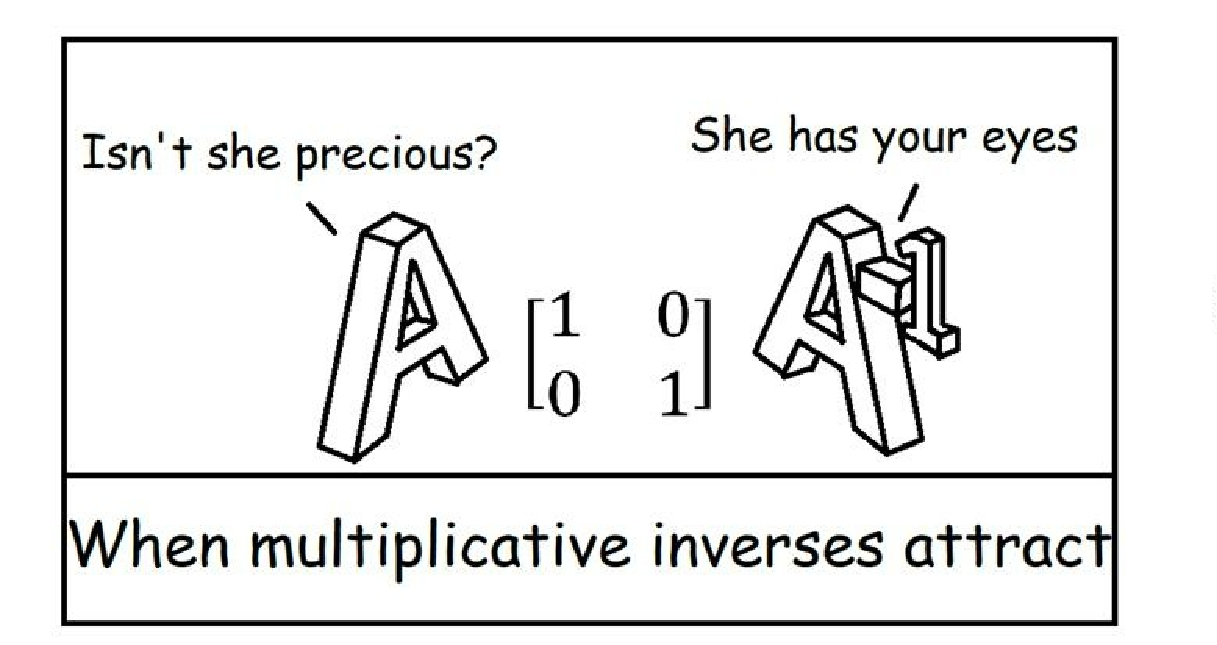
\includegraphics[scale=0.5]{Chapter3/images/attract.pdf}}
%{\vspace{-10 pt}\hfill\footnotesize (Image contributed by Thayne Hansen)}\\

\pagebreak  